\subsection{Worker f�r Daten�bermittlung}\label{subsec:Worker}
Der vorliegende Abschnitt befasst sich mit einem Teil der Wissenserwerbskomponente, der als Bindeglied zwischen den Wissenserfassungsmethoden und der Wissensbasis auftritt. In Abbildung \ref{fig:wissenserwerbskomponente} wurde dieses Bindeglied allgemein als Schnittstelle f�r die Daten�bermittlung bezeichnet. Im Rahmen dieser Studie wird von einem \textit{Worker} gesprochen, der die Aufgabe der Daten�bermittlung durchf�hren wird. Der Aufgabenbereich vom Worker l�sst sich in Abbildung \ref{fig:worker} darstellen.
\begin{figure}[H] 
	\centering
	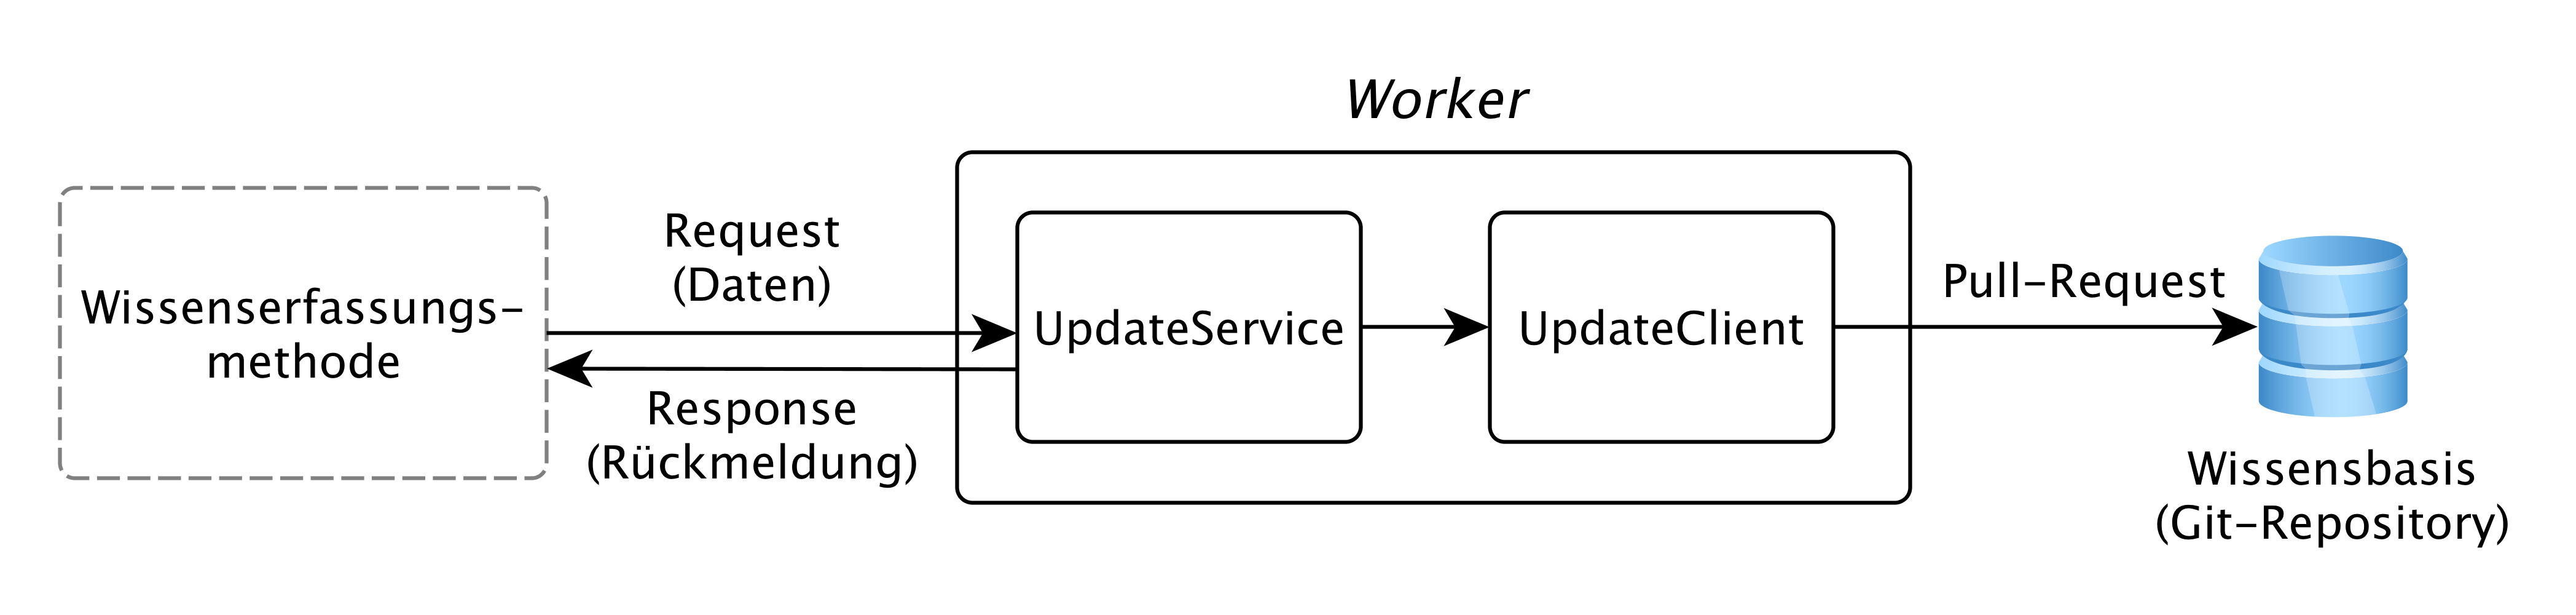
\includegraphics[width=1.0\textwidth]{images/anwendungsbereich_worker.png}
	\caption{Anwendungsbereich vom Worker}
	\label{fig:worker}
\end{figure}
In Abbildung \ref{fig:worker} sieht man, dass der Worker aus \textit{UpdateService} und \textit{UpdateClient} besteht. UpdateService stellt eine Schnittstelle dar, die f�r den Empfang der Daten zust�ndig ist. Auf der anderen Seite befasst sich UpdateClient mit der Schnittstelle der Wissensbasis (Git-Repository), um einen Pull-Request erstellen zu k�nnen.\\
Der Ablauf der Daten�bermittlung l�sst sich gem�� der Abbildung \ref{fig:worker} wie folgt beschreiben. Als erstes werden die Daten als JSON an den UpdateService geschickt (Request). Im n�chsten Schritt wird das JSON vom UpdateService verarbeitet (\glqq{}geparsed\grqq{}{}) und die Pull-Request-Erstellung an den UpdateClient delegiert. An dieser Stelle wird davon ausgegangen, dass der Pull-Request erfolgreich erstellt wurde. Der genaue Ablauf der Pull-Request-Erstellung wird im sp�teren Verlauf detaillierter angesprochen. Nachdem der Pull-Request erstellt wurde, schickt der UpdateService eine R�ckmeldung (Response) an die Wissenserfassungsmethode.\\
Die Umsetzung des Workers erfolgt auf Basis von \ac{HTTP}\footnote{https://www.w3.org/Protocols} unter Verwendung von \ac{REST}-Architekturstil, der urspr�nglich aus der Dissertation von Fielding \cite{fielding2000} stammt. Das zentrale Konzept vom Rest besteht in Ressourcen, die im globalen Raum mithilfe von \ac{URI}\footnote{https://tools.ietf.org/html/rfc3986} eindeutig identifiziert werden \cite[S.11,35]{tilkov2015}. Ein wichtiges Merkmal von REST ist die lose Kopplung zwischen dem Client und dem Server, auch als statuslose Kommunikation bezeichnet \cite[S.18]{tilkov2015}. Der Server (Worker) interessiert sich f�r den Client (Wissenserfassungsmethode) nur f�r den Zeitpunkt der Request-Verarbeitung. Danach ist der Zustand des Clients f�r den Server nicht mehr relevant.\\
Der UpdateService wird auf Basis Spark\footnote{http://sparkjava.com} umgesetzt. Spark stellt ein Micro-Framework dar, das eine kompakte, Java-basierte Implementierung von REST-API erm�glicht. Um die Daten von au�en empfangen zu k�nnen, stellt der UpdateService die \glqq{}/vendor\grqq{} Route zur Verf�gung, die vom Typ POST\footnote{https://tools.ietf.org/html/rfc7231\#section-4.3.3} ist und JSON als Medientyp erwartet.\\
Die Erstellung eines Pull-Requests erfolgt mithilfe von Github REST-API\footnote{https://developer.github.com/v3}. Diese Aufgabe wird durch den UpdateClient durchgef�hrt und setzt sich aus folgenden Schritten zusammen:
\begin{itemize}
\item[1.] \acs{SHA}-Wert vom Master-Branch holen und einen neuen Branch erstellen
\item[2.] \acs{SHA}-Wert der betroffenen JSON-Datei holen und die JSON-Datei innerhalb von Branch aktualisieren 
\item[3.] einen Pull-Request erstellen
\end{itemize}
Diese Schritte werden der UpdateClient unter Verwendung von OkHttp\footnote{https://square.github.io/okhttp} implementiert und dem UpdateService als Methoden zur Verf�gung gestellt.\\
%Im folgenden Beispiel wird der Ablauf der Aktualisierung von dargestellt 
\textit{Beispiel beschreiben}